\documentclass{standalone}
\usepackage{tikz}
\begin{document}
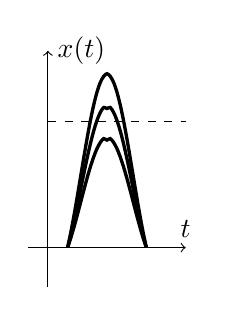
\begin{tikzpicture}[scale=2]
    \draw[->](-0.375,-0.25)--(-0.375,1.25)node[right]{$x(t)$};
    \draw[->](-0.5,0)--(0.5,0)node[above]{$t$};
    \draw[dashed](-0.375,0.8)--(0.5,0.8);
    \draw[very thick,smooth, domain=-0.25:0.25]plot(\x,{1.1*sin(4*pi*\x r)/(4*pi*\x)});
    \draw[very thick,smooth, domain=-0.25:0.25]plot(\x,{0.9*sin(4*pi*\x r)/(4*pi*\x)});
    \draw[very thick,smooth, domain=-0.25:0.25]plot(\x,{0.7*sin(4*pi*\x r)/(4*pi*\x)});
\end{tikzpicture}
\end{document}